\textbf{Acknowledgement: }{\textit{I would like to thank Dr Saulo de Oliveira for his contributions to this chapter. He kindly provided his time and expertise to generating SAINT2 structure predictions included in the analysis presented in this chapter.}

\section{Introduction}
To-date, the recommended \textit{ab initio} protein structure prediction protocol for optimal AMPLE performance is ROSETTA \cite{Keegan2015-zb, Thomas2017-sh, Thomas2015-wu, Bibby2012-lm}. This recommendation is based primarily on the superiority of the decoy quality compared to other modelling algorithms, which was recently reaffirmed by the lastest CASP12 experiments \cite{Abriata2018-lu,Ovchinnikov2017-wp}. However, \textcite{Keegan2015-zb} demonstrated that the alternative \textit{ab initio} structure prediction protocol QUARK provides a suitable alternative to ROSETTA. Although inferior in the total number of structure solutions, QUARK decoys are a suitable ROSETTA alternative in most cases \cite{Keegan2015-zb}. In particular, given ROSETTA's challenging installation procedure, availability limited to POSIX operating systems, requirement for large disk space and computationally expensive algorithm, QUARK's online server has been a very suitable alternative for AMPLE users.

Whilst ROSETTA and QUARK are amongst the best \textit{ab initio} structure prediction algorithms currently available \cite{Abriata2018-lu}, other algorithms have been developed over the last two decades \cite[e.g.,][]{Jones2001-mc,Ellis2010-zs,Adhikari2015-lb,Xu2012-jf,Marks2011-os,Wang2016-ar}. Although most of these algorithms utelise fragment-assembly algorithms similar to ROSETTA and QUARK, their procedure to fragment selection or assembly is substantially different \cite{Ellis2010-zs,Jones2001-mc}. Furthermore, predicted contact information has recently seen a spike in accuracy. This invaluable source of information is introduced differently in each protocol, and thus might have profound effects on the resulting decoy quality. In particular, physics-based algorithms relying entirely on this information are an interesting alternative to fragment-based approaches \cite{Adhikari2015-lb,Marks2011-os,Wang2016-ar}.

CONFOLD2 \cite{Adhikari2018-lj}, a distance-geometry based algorithm, utelises predicted secondary structure and contact information to rapidly generate \textit{ab initio} decoys. Unlike other algorithms, CONFOLD2's algorithm is driven almost entirely by the contact information to explore the fold space. Different contact selection thresholds are used to not limit the search space to a pre-defined selection. CONFOLD2 generates slightly inferior decoys compared to ROSETTA, however outperforms it in speed and simplicity of installation \cite{Adhikari2018-lj,Michel2017-xh}.

FRAGFOLD \cite{Jones2001-mc}, a fragment-assembly based algorithm, generates decoys in a similar fashion to ROSETTA and QUARK. However, FRAGFOLD does not rely on large structural libraries for fragment extraction. Instead, it provides a relatively small library of supersecondary structural fragments and short length fragments, which were extracted from high resolution protein structures. Since the generalised fragment library is shipped with FRAGFOLD and target-specific fragments extracted based on secondary structure and a sequence-based threading score, it enables fast and easy fragment library generation compared to ROSETTA \cite{Kosciolek2014-bt}.

SAINT2 \cite{De_Oliveira2017-sg}, a further fragment-assembly based algorithm is substantially different to most others. SAINT2 attempts \textit{ab initio} structure prediction sequentially, starting from either either terminus of the target sequence \cite{De_Oliveira2017-sg}. Furthermore, SAINT2 uses FLIB \cite{De_Oliveira2015-kb} for fragment picking, an algorithm shown to outperform ROSETTA's equivalent NNMake \cite{Gront2011-sv} in precision with very similar coverage. 

Since some of these algorithms are readily available and often easier to install without the overhead of large databases for fragment picking, the work in this study focused on exploring three alternative \textit{ab initio} structure prediction algorithms and their value in unconventional \gls{mr}. The \textit{ab initio} structure prediction protocols CONFOLD2 \cite{Adhikari2018-lj}, FRAGFOLD \cite{Jones2001-mc} and SAINT2 \cite{De_Oliveira2017-sg}, were explored given their substantially different approaches to AMPLE's current default ROSETTA \cite{Rohl2004-dj}.

\section{Materials \& Methods}
\subsection{Target selection}
This study was conducted using all 27 targets from the PREDICTORS dataset (\cref{sec:methods_dataset_predictors}). 

\subsection{Contact prediction}
Residue-residue contact information for 18 out of 27 targets were predicted using METAPSICOV v1.04 \cite{Jones2015-vq}. 

Secondary structure and solvent exposure were predicted using PSIPRED v4.0 \cite{Jones1999-ed} and SOLVPRED (shipped with METAPSICOV v1.04), respectively. The \gls{msa} for coevolution-based contact prediction was generated using HHBLITS \cite{Remmert2011-kt} against the \texttt{uniprot20\_2016\_02} database. CCMPRED v0.3.2 \cite{Seemayer2014-zp}, FREECONTACT v1.0.21 \cite{Kajan2014-bx} and PSICOV v2.1b3 \cite{Jones2012-ks} were used by METAPSICOV to generate contact predictions.

METAPSICOV STAGE 1 contact predictions were used in \textit{ab initio} structure prediction since those result in more accurate structure predictions \cite{Jones2015-vq}.

\subsection{\textit{Ab initio} structure prediction} \label{sec:ample_saint2_modelling}
The ROSETTA 3- and 9-residue fragment libraries for each target were generated using the ROBETTA online server (\url{http://robetta.bakerlab.org/}). The option to ``Exclude Homologues'' was selected to avoid inclusion of homologous fragments. Each target sequence and its fragments were subjected to ROSETTA v2015.22.57859 \cite{Rohl2004-dj} and 1,000 decoys per target generated with AMPLE v1.2.0 ROSETTA default options. Top-$L$ contact pairs were used in combination with the \textit{FADE} ROSETTA energy function, identical to the benchmark outlined in \cref{chap:alternate_abinitio_protocols}.

The CONFOLD2 decoys were generated using CONFOLD2 v2.0 \cite{Adhikari2018-lj} and \gls{cns} v1.3 \cite{Brunger1998-sz}. Default parameters were used except for the number of decoys per run, which was increased from 20 to 25 with \texttt{-mcount 25}. This resulted in 40 seperated runs differing only in the number contact pairs used, which was increased by 0.1 from $L/10$ to $4L$.

The FRAGFOLD decoys were generated using FRAGFOLD v4.80 \cite{Jones2001-mc} with default options. Homologous fragments were removed from the shipped library  by excluding all entries with \gls{pdb} identifiers identical to those retrieved from the ROBETTA server. All contact pairs were used according to FRAGFOLD's internal protocol.

The fragment libraries for SAINT2 were generated using FLIB \cite{De_Oliveira2015-kb}, which generates on average ~30 fragments per target position that are 6 to 20 residues long. Homologous fragments were removed from the final fragment list using the \gls{pdb} identifiers obtained from the ROBETTA online server. The secondary structure prediction and solvent accessibility scores were also obtained from the ROBETTA server. SAINT2 was used for decoy generation, and ~1,000 decoys generated per target. The procedure and parameters were identical to those described in Supplementary Information (p. 16) by \textcite{De_Oliveira2017-sg}.

\subsection{Molecular Replacement}
All decoy sets were subjected to AMPLE v1.2.0 and CCP4 v7.0.28. Default options were chosen with the following exceptions: decoys in all 10 clusters were used, subcluster radii thresholds were set to 1 and 3\AA, and side-chain treatments were set to \texttt{polyala} only. This change in protocol from AMPLE's initial mode of operation \cite{Bibby2012-lm} was shown to be advantageous in most cases by \textcite{Thomas2017-qu}, and thus trialled in this context.  Each \gls{mr} run was assessed using the criteria defined in \cref{sec:methods_mr_success}.

\section{Results}
The purpose of this study was to investigate the usefulness of alternative \textit{ab initio} structure prediction in AMPLE. Three promising leads widely used in the \textit{ab initio} modelling experiments were examined and compared against AMPLE's current algorithm of choice. This led to a direct comparison of the algorithms ROSETTA \cite{Rohl2004-dj}, CONFOLD2 \cite{Adhikari2018-lj}, FRAGFOLD \cite{Jones2001-mc} and SAINT2 \cite{De_Oliveira2017-sg}. All four algorithms have recently seen great improvements through the use of residue-residue contact information, which predicted using the METAPSICOV \cite{Jones2015-vq} algorithm.

\subsection{Alignment depth and contact prediction precision}
The first step in this study was the prediction of residue-residue contacts using the metapredictor METAPSICOV for 18 targets in the PREDICTORS dataset \cite{Jones2015-vq}. Since we attempted to test each of the structure prediction boundaries in extreme cases, a variety of targets with different alignment depths were chosen. The alignment depth of METAPSICOV-generated HHBLITS alignments ranges from 6 to 6,186 across all targets (\cref{fig:ample_saint2_alndepth}). Five targets contain alignments with a depth of less than 200, a rough threshold to indicate suitability of a \gls{msa} for coevolution-based contact prediction (\cite{Simkovic2017-xs}). A further six targets contain at least 200 and less than 1000 sufficiently-diverse sequences, whilst for the remaining 16 targets the \gls{msa} depth is at least 1,000.

\begin{figure}[H]
    \centering
    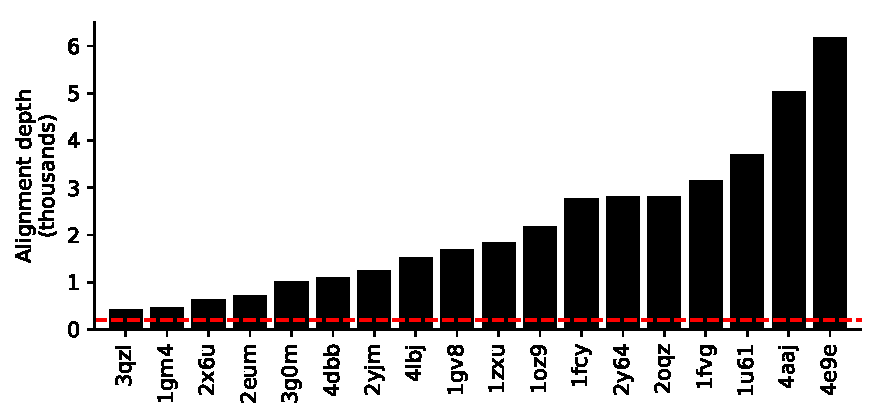
\includegraphics[width=\textwidth]{ample_saint2_alndepth.pdf}
    \caption[Distribution of alignment depth for subset of targets in the PREDICTORS dataset.]{Distribution of HHBLITS alignment depth for subset of targets in the PREDICTORS dataset. Red line indicates alignment depth threshold of 200 sequences.}
    \label{fig:ample_saint2_alndepth}
\end{figure}

Coevolution-based contact predictors rely heavily on the alignment depth for accurate contact predictions. In this work, these findings are further confirmed. Sequence alignments with depths of less than 1000 sequences highlight lower precision scores across a number of cutoffs compared to those with deeper alignments (\cref{fig:ample_saint2_conprec}). Given the alignment depths and top-$L$ contact predictions, a significant positive correlation between the two is found (Spearman's $\rho=0.57$, p-value $<0.02$). A moving average analysis shows that those contact predictions based on alignments with more than 1000 effective sequences yield better precision scores of at least 0.09 units up to 0.34 units. The difference between the two moving average curves highlights that the difference is greater at lower cutoff values, i.e. only the very best contacts are included in the selection. This difference declines more drastically for targets with deeper alignments (\cref{fig:ample_saint2_conprec}).

\begin{figure}[H]
    \centering
    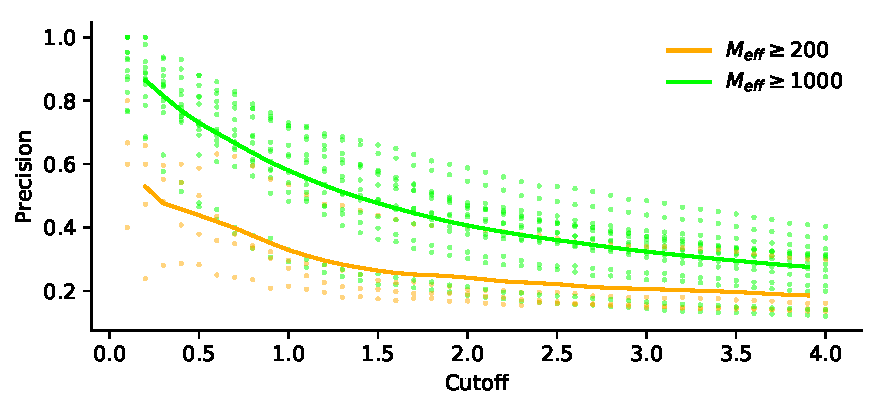
\includegraphics[width=\textwidth]{ample_saint2_conprec.pdf}
    \caption[Contact predicion analysis for numerous contact selection cutoffs]{Contact precision analysis for numerous contact selection cutoffs for targets with alignment depths of more than 200 and more than 1000 sequences. Lines indicate moving averages for both categories with a window size of three residues. $M_{eff}$ refers to the alignment depth (number of effective sequences).}
    \label{fig:ample_saint2_conprec}
\end{figure}

\subsection{Comparison of decoy quality}
One main interest of the work presented in this chapter is the comparison of the quality of decoys predicted with four \textit{ab initio} structure prediction algorithms. To-date, no such direct comparison exists on the same dataset, and thus might provide direct insights into the performance of each.

\begin{figure}[H]
    \centering
    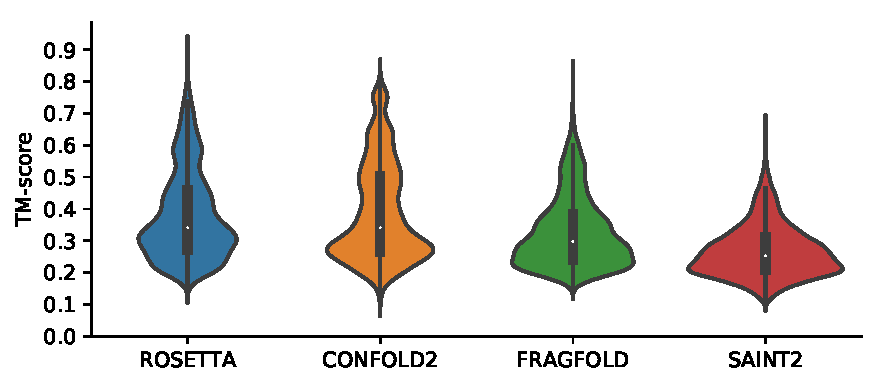
\includegraphics[width=\textwidth]{ample_saint2_tmscoredist.pdf}
    \caption[Distribution of decoy TM-scores for four modelling algorithms]{Kernel Density Estimate of decoy TM-scores for four different \textit{ab initio} structure prediction algorithms, namely ROSETTA, CONFOLD2, FRAGFOLD and SAINT2. CONFOLD2 contains 9,000 less decoys than the remaining algorithms (for further details refer to \cref{sec:ample_saint2_modelling}).}
    \label{fig:ample_saint2_tmscoredist}
\end{figure}

An initial comparison of overall performance highlights that ROSETTA generates the highest quality decoys (\cref{fig:ample_saint2_tmscoredist}). Across all modelling algorithms the distribution of TM-scores right-skewed, which indicates a higher proportion of non-native-like folds within the sets. A TM-score quantile evaluation of each decoy set by algorithm shows that ROSETTA and CONFOLD2 contain only a single set with a lower quantile of less than 0.2 TM-score units. In comparison, FRAGFOLD predicted three and SAINT2 eight decoy sets with a lower quantile of less than the aforementioned threshold. In comparison, ROSETTA, CONFOLD2 and FRAGFOLD predicted six, seven and five decoy sets with upper quantiles greater than 0.5 TM-score units, whilst SAINT2 predicted zero. 

A direct comparison of the methods by median TM-score of each contact-assisted decoy set reaffirms ROSETTA's performance in predicting \textit{ab initio} decoys accurately. Across 18 targets, ROSETTA decoy sets contain the best median TM-score for 11 targets (CONFOLD2 for remaining seven targets). This is further strengthened when comparing the top-1 decoy for which ROSETTA predicts the best in 13 cases (CONFOLD2 in three cases, FRAGFOLD and SAINT2 in one) (\cref{fig:ample_saint2_tmscoredataincl}).

\begin{figure}[H]
    \centering
    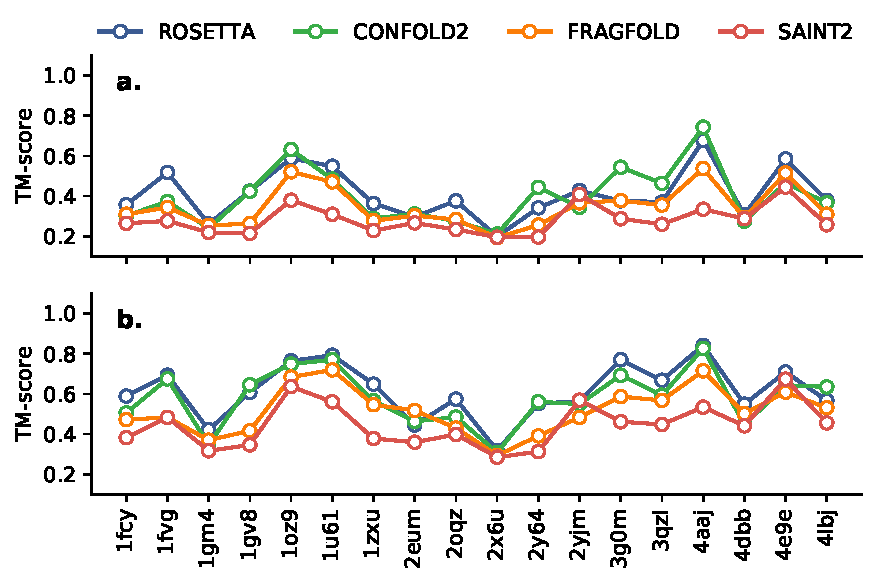
\includegraphics[width=\textwidth]{ample_saint2_tmscoredataincl.pdf}
    \caption[Per-target TM-score analysis for four modelling algorithms with contacts]{Per-target TM-score analysis for targets modelled with contact information and four separate \textit{ab initio} structure prediction algorithms. Analysis is subdivided by (a) median TM-score of all decoys in each set and (b) TM-score of the top-1 decoy in each set.}
    \label{fig:ample_saint2_tmscoredataincl}
\end{figure}

\textcite{Abriata2018-lu} recently attributed the success in the CASP12 experiments to improved accuracy of coevolution-based contact predictors and the availability of many more sequence homologs than ever before. Thus, it is of great interest to explore the structure prediction algorithms in this study with regards to their dependence on the availability of sequence homologs and precise contact predictions.

The results obtained in this study further support the conclusions made by \textcite{Abriata2018-lu} but only for the ROSETTA algorithm. A Spearman's rank-order \gls{cc} analysis of alignment depth and median TM-score shows a significant positive correlation for ROSETTA-generated decoy sets (Spearman's $\rho=0.68$, $p<0.01$). This positive correlation is also found for ROSETTA-generated decoy sets with regards to their top-$L$ precision and median TM-score (Spearman's $\rho=0.61$, $p<0.01$). All other modelling algorithms do not show a significant correlation, although better decoy sets are generally obtained with greater alignment depths and more precise top-$L$ contacts (\cref{fig:ample_saint2_neffprectm}). Furthermore, the sample size for each correlation analysis was small ($n=18$), and thus further test cases are required for a more confident inference.

\begin{figure}[H]
    \centering
    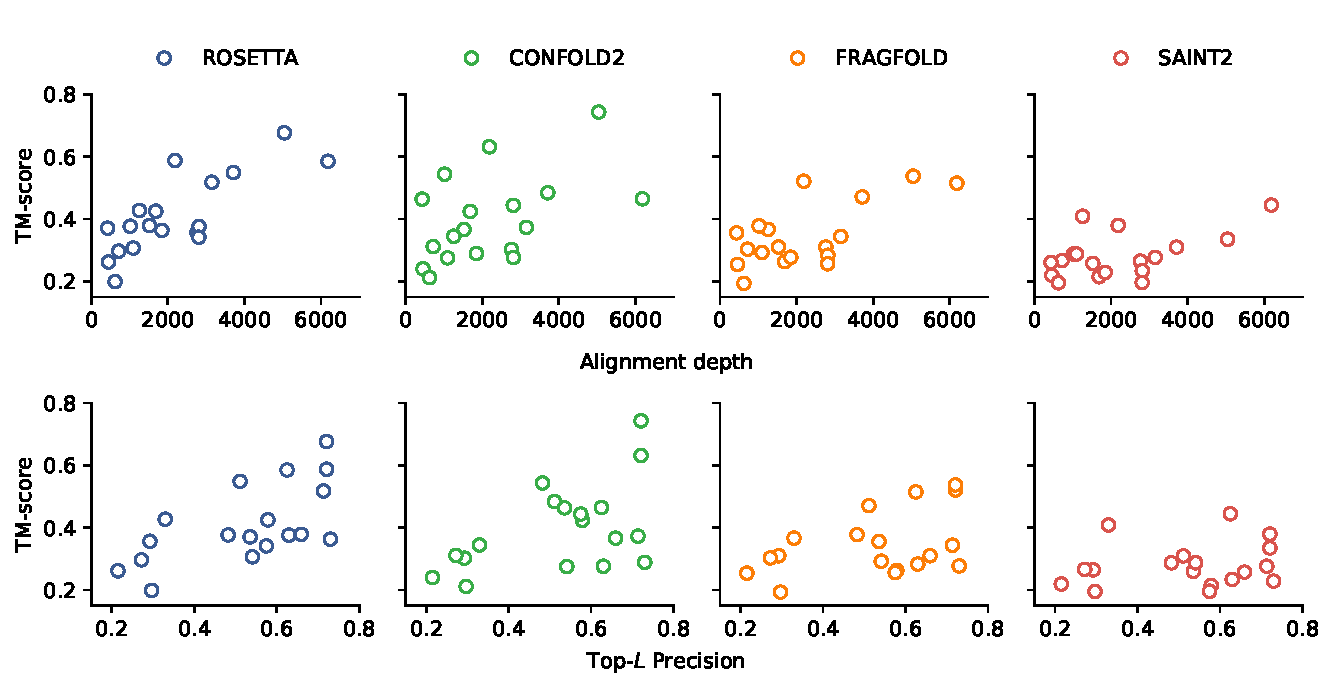
\includegraphics[width=\textwidth]{ample_saint2_neffprectm.pdf}
    \caption[Analysis of alignment depth, precision and TM-scores]{Analysis of median TM-scores of the contact-based decoy sets and their dependence on  alignment depth and top-$L$ precision.}
    \label{fig:ample_saint2_neffprectm}
\end{figure}

Beyond the use of contact information, parts of this study explored the performance of ROSETTA, FRAGFOLD and SAINT2 when no contact information is provided as distance restraints in \textit{ab initio} structure prediction (CONFOLD2 requires contact information, and thus was excluded). ROSETTA performs best for seven of the nine contact-free decoy sets based on median TM-score of the entire decoy set and the TM-score of the top-1 decoy (\cref{fig:ample_saint2_tmscoredataexcl}). However, the difference is marginal for the majority of cases. The median values for eight ROSETTA and FRAGFOLD decoy sets differ by less than 0.10 TM-score units (seven ROSETTA and SAINT2 sets by less than 0.10 units). Furthermore, the top-1 decoys for only three targets differ greatly between the modelling algorithms, whilst the rest is near identical between algorithms (\cref{fig:ample_saint2_tmscoredataexcl}). 

The top decoy predicted by ROSETTA and SAINT2 based on the sequence of the FAT domain of focal adhesion kinase (\gls{pdb} ID: 1k40) differs by 0.35 TM-score units. More significantly though, the top decoy predicted by ROSETTA for the outer surface protein A (\gls{pdb} ID: 2ol8) is considered native-like (TM-score $=0.59$), whilst the FRAGFOLD (TM-score $=0.35$) and SAINT2 (TM-score $=0.24$) counterparts predict incorrect folds. A near-identical scenario applies to the top decoys of the Hypothetical protein PF0907 (\gls{pdb} ID: 4pgo) (ROSETTA TM-score $=0.68$; FRAGFOLD TM-score $=0.27$; SAINT2 TM-score $=0.39$).

\begin{figure}[H]
    \centering
    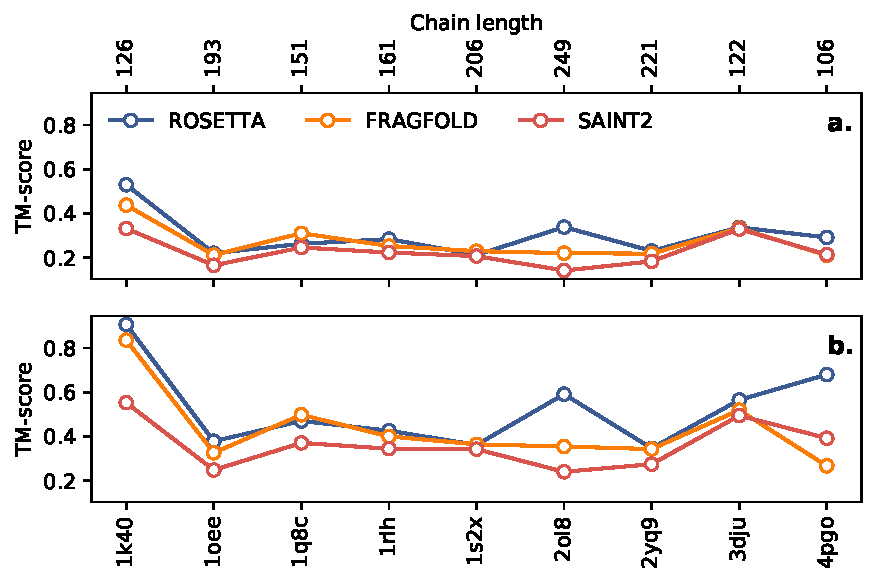
\includegraphics[width=\textwidth]{ample_saint2_tmscoredataexcl.pdf}
    \caption[Per-target TM-score analysis for four modelling algorithms without contacts]{Per-target TM-score analysis for targets modelled without contact information and four separate \textit{ab initio} structure prediction algorithms. Analysis is subdivided by (a) median TM-score of all decoys in each set and (b) TM-score of the top-1 decoy in each set.}
    \label{fig:ample_saint2_tmscoredataexcl}
\end{figure}

An analysis of the modelling results by target fold shows that all-\textalpha\ and mixed \textalpha-\textbeta\ target folds are less challenging to predict than all-\textbeta\ targets (\cref{fig:ample_saint2_tmfoldsize}). The multimodal distributions of all-\textalpha\ and mixed \textalpha-\textbeta\ target decoys predicted by ROSETTA spans from 0.10 TM-score units to 0.80. In comparison, the roughly normal distribution for all-\textbeta\ by the same algorithm centres at 0.32 TM-score units (s.d.=0.08 TM-score units). Similarly, FRAGFOLD decoys show a more spread distribution of decoys for all-\textalpha\ and mixed \textalpha-\textbeta\ decoys compared to all-\textbeta. Although the multimodal distribution of TM-scores for all-\textbeta\ target decoys might indicate better performance for some targets, it is most certainly misleading since three all-\textbeta\ targets are missing from the dataset in comparison to the other algorithms. Lastly, the distributions of TM-scores for either fold class of SAINT2 decoys appear more similar than the others indicating less difference between the fold classes. However, similarly to the ROSETTA decoys the all-\textbeta\ distribution appears normal whilst the other two are right-skewed highlighting some more accurate decoys in the overall set.

\begin{figure}[H]
    \centering
    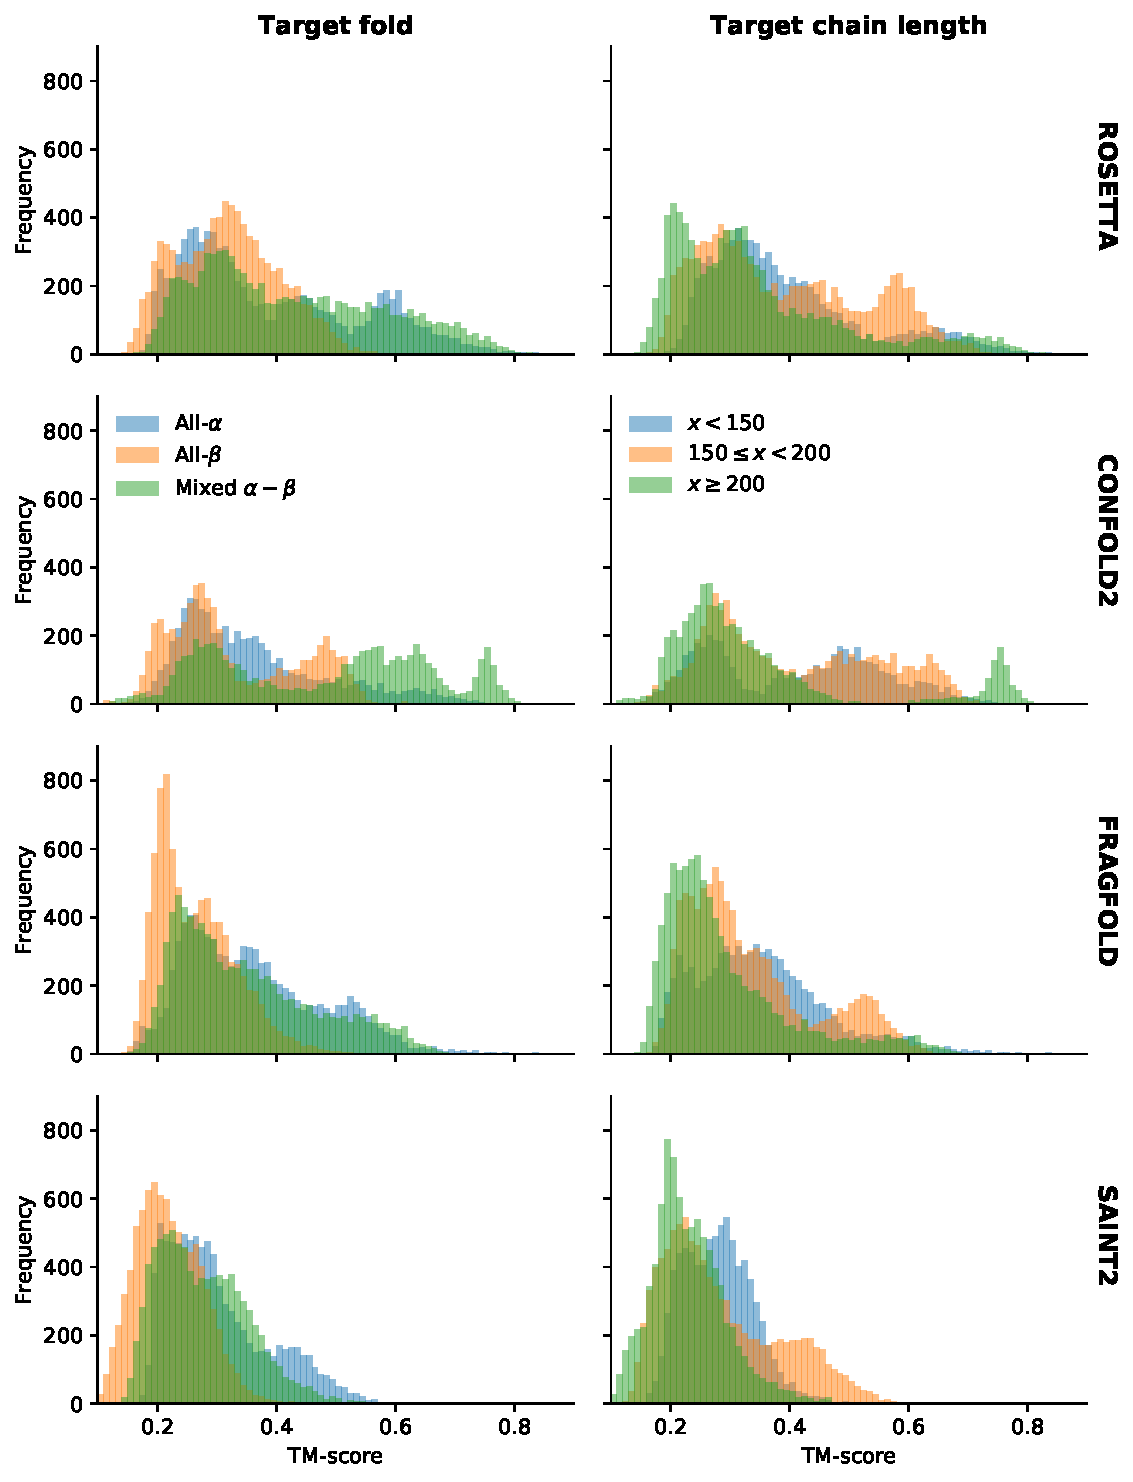
\includegraphics[width=\textwidth]{ample_saint2_tmfoldsize.pdf}
    \caption{Distribution of decoy TM-scores by fold, chain length and algorithm.}
    \label{fig:ample_saint2_tmfoldsize}
\end{figure}

A further subdivision of all target decoys is by target chain length. At the stage of target selection, three main bins were defined from which targets were randomly sampled (see \cref{sec:methods_dataset_predictors}). These bins were defined with target chain length edges of 150 and 200 creating three bins: $0 < x < 150$ \& $150 \leq x < 200$ \& $x \geq 200$ ($x$ refers to the target chain length). A grouping of the decoy TM-scores by algorithm and target chain length indicates little difference in modelling difficulty (\cref{fig:ample_saint2_tmfoldsize}). Each of the modelling algorithms shows the largest spread for targets with chain lengths in the bin $150 \leq x < 200$. Surprisingly, only FRAGFOLD and SAINT2 performed better for targets in the smallest bin size whilst CONFOLD2 found those targets most challenging. CONFOLD2 also generated the best decoys for one of the largest targets in the dataset. The set of CONFOLD2 decoys for N-(5-phosphoribosyl)anthranilate isomerase (\gls{pdb} ID: 4aaj) have a median TM-score of 0.74 units. ROSETTA decoys show a comparable median TM-score of 0.68; however, FRAGFOLD (median TM-score=0.54) and SAINT2 (median TM-score=0.33) were unable to generate decoys of similarly high quality.

\subsection{Molecular Replacement}
Each \textit{ab initio} structure prediction algorithm generated decoy sets, which are sufficient for structure solution (\cref{fig:ample_saint2_mrsuccess}). ROSETTA and SAINT2 decoy sets led to five structure solutions each, whilst FRAGFOLD decoys to four and CONFOLD2 decoys to two. All four algorithms predicted decoys of good enough quality to solve the structures of the Hypothetical protein AQ\_1354 (\gls{pdb} ID: 1oz9) and Putative Ribonuclease III (\gls{pdb} ID: 1u61), although SAINT2-based AMPLE search models yielded the highest ratio of successful search models in both cases (\cref{fig:ample_saint2_mrsuccess}). Besides these two targets, little consensus exists amongst the targets for which structure solutions were obtained.

\begin{figure}[H]
    \centering
    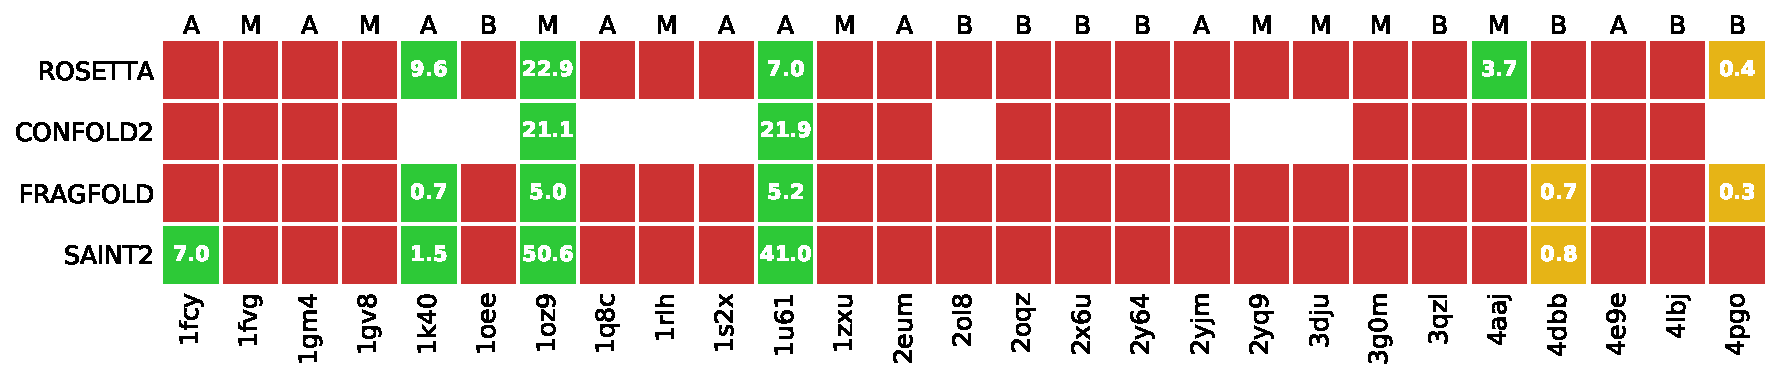
\includegraphics[width=\textwidth]{ample_saint2_mrsuccess.pdf}
    \caption[Summary of MR success with AMPLE ensemble search models.]{Summary of MR success with AMPLE ensemble search models. Search models are based on decoy sets generated with different \textit{ab initio} structure prediction protocols. The colour coding indicates structure solution: no solution (red), one solution (orange), more than one solution (green). The number in cells with at least one solution states the percentage successful search models.}
    \label{fig:ample_saint2_mrsuccess}
\end{figure}
